\section{Discussion}
\label{sec:discussion}

% In this section we discuss how the idea of auxiliary histories, which
% can store observed thread interference, can be applied to reason
% quantitatively about other non-linearizable concurrent structures.
%

% \paragraph{Balancer-based concurrent container implementations}

% In Section~\ref{sec:counting}, we have shown how one can reason
% quantitatively about behavior of a counting network, implemented via a
% balancer, using histories, whose entries snapshot interference,
% therefore characterizing the out-of-order discrepancies between its
% results.

\paragraph{Reasoning about quantitatively quiescent queues}

The idea of interference-capturing histories, which allowed us to
characterize the out-of-order discrepancies between the results of a
counting network in Section~\ref{sec:counting},
%
can be applied to specify other balancer-based data structures, for
instance, queues~\cite{Derrick-al:FM14}.
%
The picture on the right illustrates schematically a non-linearizable
queue~\cite{Derrick-al:FM14}, which is built out of 
%
\begin{wrapfigure}[6]{r,trim}[-45pt]{1.5cm}   
\centering 
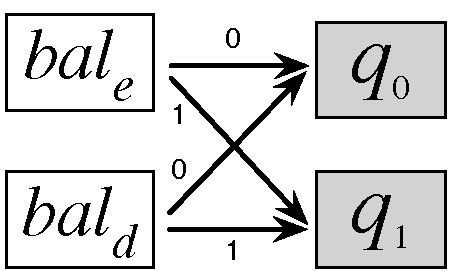
\includegraphics[width=3.0cm]{queue.pdf} 
\end{wrapfigure}
%
two \emph{atomic} queues, $q_0$ and $q_1$, and two
balancers, $\bal_e$ and $\bal_d$.  The balancers are used to
distribute the workload between the two queues by directing the
threads willing to enqueue and dequeue elements, correspondingly.

%Taking inspiration from the development in Section~\ref{sec:counting},
%
One can think of representing the pending enqueue/dequeue requests to
each of the two queues, $q_0$ and $q_1$, by two separate sets of
tokens, as shown in Figure~\ref{fig:chist2}.
%
The white and gray boxes correspond to the present and
dequeued nodes in the queue in the order they were added/removed.
%
Therefore, white elements are those that are currently in the queue.
%
Similarly, the white-colored tokens are for enqueueing elements, so
the elements $x$, $y$, $z$ and $k$ are going to be added to the
corresponding atomic queues. Gray-colored tokens correspond to
dequeueing capabilities for one or another atomic queue, distributed
among the threads, so the elements $c$ and $d$ are going to be removed
next, on the expense of the corresponding dequeue tokens.
%
The timestamps of the entries in the queue history, omitted from the
figure, are created, as elements are being enqueued to $q_0$ and
$q_1$, and the parity of a timestamp corresponds to the atomic queue
being changed. Thus, there might be ``gaps'' in the combined queue
history reminiscent to the gaps in the counter history from
Section~\ref{sec:counting} (\eg, the gap caused by the absence of an
``even'' element in the combined history right between $d$ and $e$ in
Figure~\ref{fig:chist2}, as indicated by ``?''), which will cause
out-of-order anomalies during concurrent executions.
%
%
By accounting for the number of past and present tokens for enqueueing
and dequeueing, one should be able to capture the effects of
interference and express a quantitative boundary on the discrepancy
between the results, coming out of order.

{
\setlength{\belowcaptionskip}{-10pt}
\begin{figure}[t]
\centering
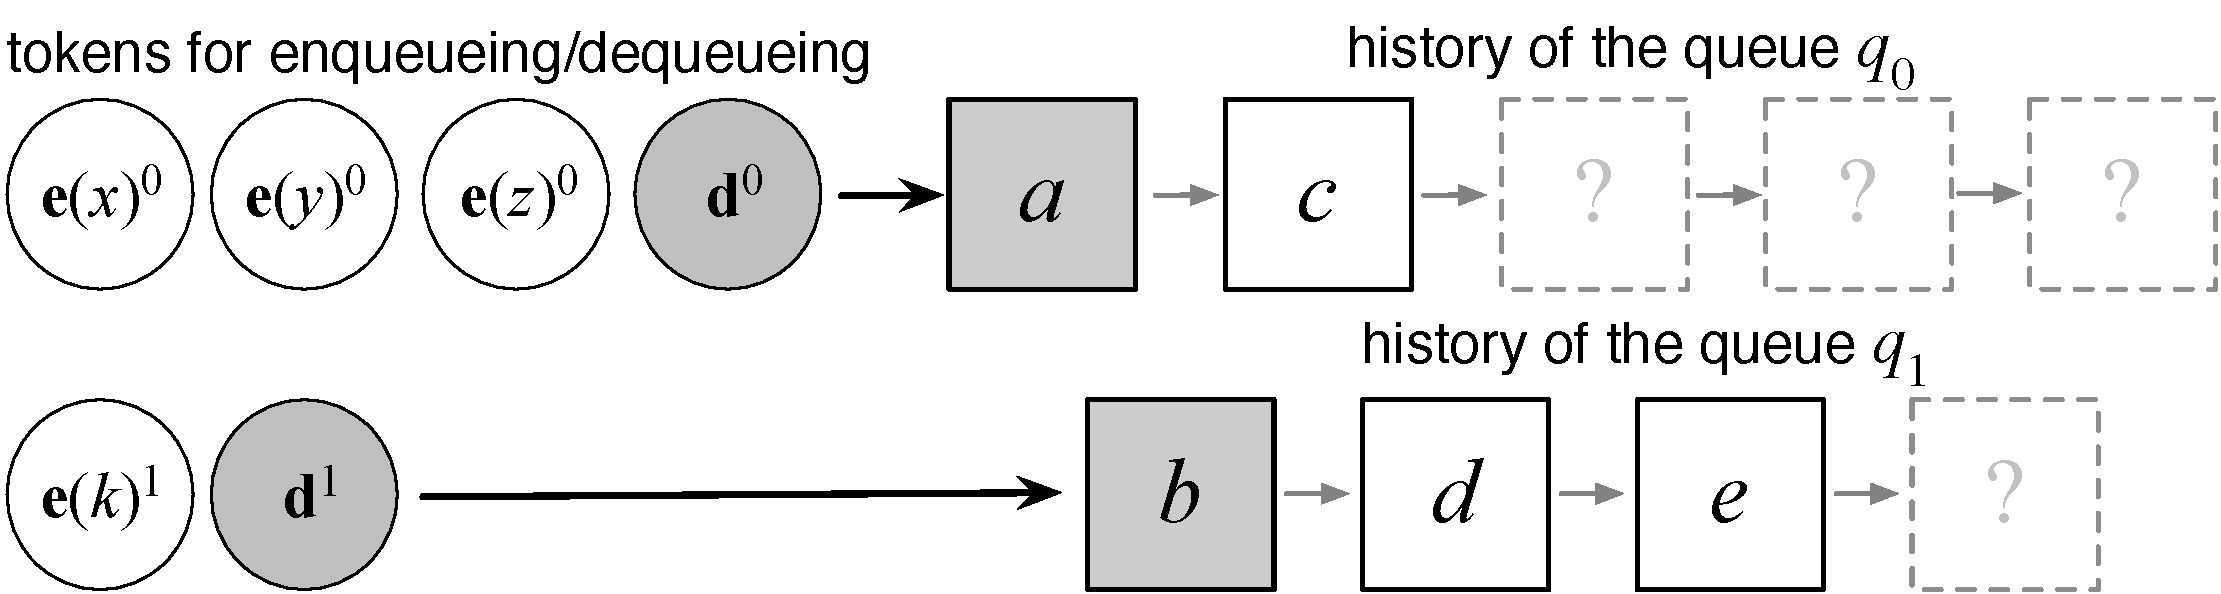
\includegraphics[width=8.2cm]{chist2.pdf}      
\caption{Tokens and histories of a balancer-based queue.}
\label{fig:chist2}
\end{figure}
}

% , in terms of ordering of
% timestamps, assigned to enqueue/dequeue events in the combined queue
% history.

% The intuition is similar in the case of balancer-based
% stacks~\cite{Jagadeesan-Riely:ICALP14}, with the main difference being
% that the elements are removed in a LIFO order and, hence, the
% \emph{rightmost} entries of a corresponding partial (\ie, even or odd)
% history are painted gray first.
% %
% We leave complete formalization of these structures to the future
% work.

% \paragraph{In defense of compositional reasoning}

% \todo{cite Lamport ane elaborate.}

\paragraph{How much information to expose in a spec?}
\label{sec:how-much-information}

The specs we have proved for concurrent objects in
Sections~\ref{sec:overview} and~\ref{sec:counting} allow for efficient
compositional reasoning about clients, but they are also non-trivial
to formulate and verify. Luckily, the FCSL way of reasoning provides a
flexible solution for the compositionality-versus-complexity
conundrum~\cite[\S 7]{Lamport:COMPOS97}.

In FCSL, it is up to the library implementor to decide, how much of
implementation-specific insight should go into a spec. The amount of
such details is determined based on the foreseen client scenarios. For
instance, we have hidden the balancer in the spec~\eqref{eq:qc-spec},
but decided keep the exact constant $2$, which would allow us to
derive more precise quantitative bounds later (see
Section~\ref{sec:qqc-client}). However, we could have hidden this
component too (as well as, for instance, some parts of the invariant
$\ic$), by employing in the specification sigma-types (a
dependently-typed analogue of existential types), provided by FCSL as
it's embedded into Coq~\cite{Coq-manual}. We could have also omitted
tokens from the spec, therefore, reducing the set of derivable
client-specific properties to Section~\ref{sec:counting}'s~\textbf{R1}
only.


